\documentclass[12pt]{article}
\usepackage[utf8]{inputenc}
\usepackage[margin=1in]{geometry}
\usepackage[spanish]{babel}\decimalpoint
\usepackage{setspace}\onehalfspacing
\usepackage{parskip} % Espacio entre parrafos.
\usepackage{graphicx} % Para usar comando \includegraphics[]{}
\usepackage{amssymb} % Para usar el simbolo del conj. de los Reales.
\usepackage{amsmath} % Para usar columnas vectoriales.
\usepackage{multirow} % Para unir multiples filas en una tabla.
\usepackage{hyperref} % Siempre debe ser el ultimo paquete.


\setcounter{tocdepth}{2} % Que no incluya subsubsections en la tabla de contenidos (toc).

%================================

\title{Clase 21: Aplicación de las Integrales: Nuevas Funciones y Áreas entre dos Curvas.}
\author{MIT 18.01: Single Variable Calculus.}
\date{}

\begin{document}

\maketitle

\begin{abstract}
\noindent Desde esta clase comenzaremos a ver aplicaciones de la integral. En primer lugar, usaremos el TFC 2 para continuar buscando nuevas funciones a partir de ella. Luego, ayudados del TFC 1 calcularemos el área que se genera entre dos curvas.
\end{abstract}

\section{Buscando funciones ``nuevas'' (continuación).}

\subsection{Función Logaritmo.}

En la clase anterior resolvimos la siguiente ecuación diferencial:
\[
  y' = \frac{1}{x}
\]
a partir del TFC 2 y teniendo como condición inicial $L(1) = 0$:
\[
  L(x) = \int_{1}^{x} \frac{1}{t}dt
\]
También señalamos que estas funciones resultantes son ``nuevas'' o que no pueden ser expresadas en forma de otras ya conocidas.

Ahora vamos a usar a esta $L(x)$ como la definición del logaritmo y buscaremos sus propiedades a partir de esta función, que está en forma de integral.

Intentemos conocer la forma de $L(x)$. Por medio del TFC 2 podemos asegurarnos que:
\[
  L'(x) = \frac{1}{x}
\]
Como vemos, $L'(x)$ no puede ser igual a cero, por lo que no tiene puntos críticos. Por otra parte, en el punto de la condición inicial, $L'(1) = 1$. De hecho, en general:
\[
  L'(x) = \frac{1}{x}
    \left\{
      \begin{aligned}
      x < 0, \ L'(x) < 0 \\
      x > 0, \ L'(x) > 0
      \end{aligned}
    \right.
\]
Lo que nos muestra cuándo $L(x)$ crece o decrece.

También podemos ver la concavidad de $L(x)$ a partir de su segunda derivada:
\[
  L''(x) = \frac{-1}{x^{2}}
\]
Al igual que $L'(x)$, $L''(x)$ no puede ser igual a cero y, además, siempre será negativa, lo que implica que $L(x)$ no tiene puntos de inflexión y es cóncava hacia abajo para todo $x$ en los $\mathbb{R}$.

En cuanto a sus límites, $L(x) \to -\infty$ a medida que $x \to 0$ y, mientras $x \to \infty$, $L(x) \to \infty$.

Por medio de $L(x)$ también podemos \textbf{definir el número} $e$ como un valor tal que $L(e) = 1$.

A continuación tenemos una gráfica de $L(x)$ que considera toda la información que recopilamos más la definición de $e$.

\begin{figure}[hbt!]
\centering
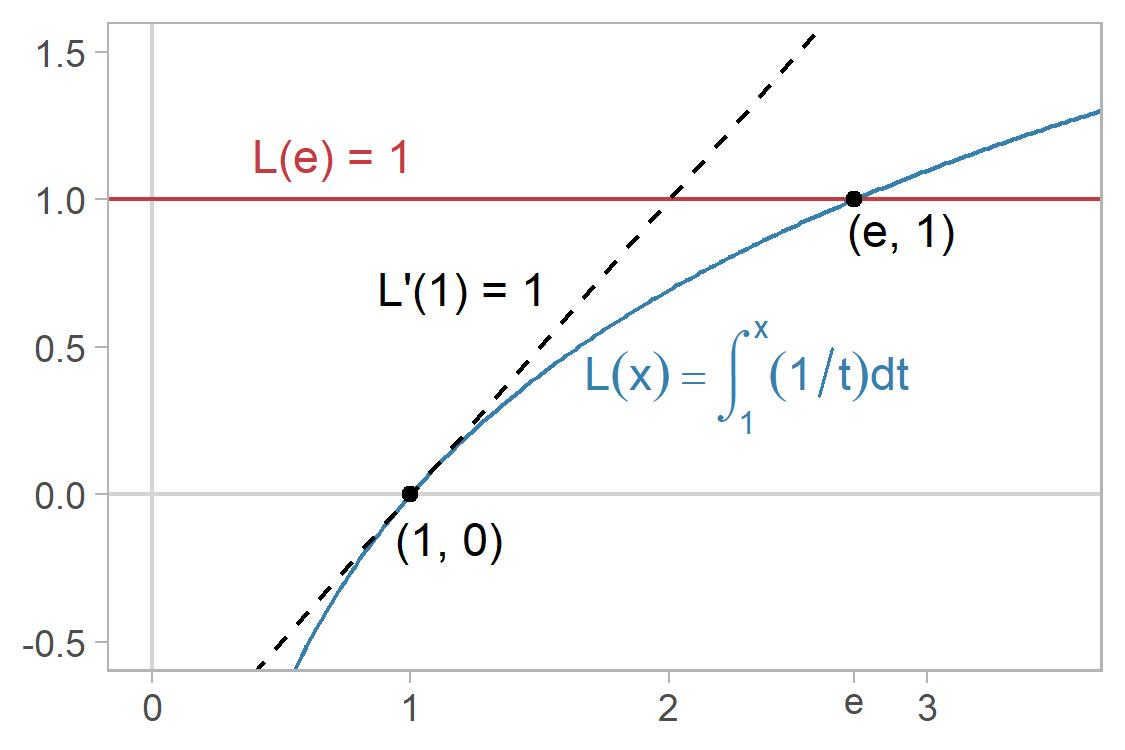
\includegraphics[scale=0.7]{img/log_int_plot.jpg}
\end{figure}

Veamos que $L(x) < 0$ cuando $0 < x < 1$. Un motivo es que $L(1) = 0$ y que es una función creciente. Pero otra razón se da a partir de una de las propiedades de las integrales:
\[
  L(x) = \int_{1}^{x} \frac{1}{t}dt = - \int_{x}^{1} \frac{1}{t}dt < 0
\]
El lado derecho de la igualdad derecha es correcta porque:
\[
  \int_{x}^{1} \frac{1}{t}dt > 0
\]
puesto que $x < 1$, lo que es dado por el orden de los límites. En consecuencia:
\[
  -\int_{x}^{1} \frac{1}{t}dt < 0
\]
Ahora, a partir de $L(x)$, tratemos de demostrar la siguiente igualdad:
\[
  L(ab) = L(a) + L(b)
\]
La función $L(ab)$ podemos escribirla a partir de la definición de $L(x)$ y podemos igualarla como una suma de ella misma descompuesta en dos integrales:
\[
  \int_{1}^{ab} \frac{1}{t}dt = \int_{1}^{a} \frac{1}{t}dt + \int_{a}^{ab} \frac{1}{t}dt
\]
Observemos que al menos se cumple que:
\begin{align*}
  L(ab) &= \int_{1}^{ab} \frac{1}{t}dt & L(a) &= \int_{1}^{a} \frac{1}{t}dt 
\end{align*}
Nos falta ver si, efectivamente:
\[
  L(b) \overset{\text{??}}{=} \int_{a}^{ab} \frac{1}{t}dt
\]
Para ello, usemos el método de cambio de variables a partir de los límites de la integral del lado derecho. Veamos que ambos son múltiplos de $a$ ($a$ y $ab$). Por lo tanto, como estrategia podemos establecer que:
\begin{align*}
  t &= au & dt &= adu
\end{align*}
donde $u$ es la nueva variable que usaremos.

Recordemos que, al cambiar variables, no solo escribimos de forma distinta lo que está adentro de la integral, sino que también sus límites. Como $t = au$, entonces para que $t = a$, $u = 1$. Así mismo, para que $t = ab$, $u = b$. Por consiguiente:
\[
  L(b) = \int_{a}^{ab} \frac{1}{t}dt = \int_{1}^{b} \frac{1}{au}adu = \int_{1}^{b} \frac{1}{u}du
\]
Así, demostramos que $L(ab) = L(a) + L(b)$, la cual es la propiedad de los logaritmos $\ln(ab) = \ln(a) + \ln(b)$.

\subsection{Función Error.}

Otra función nueva que analizaremos, es:
\[
  L(x) = \int_{0}^{x} e^{-t^{2}} dt
\]

Por el TFC 2, podemos afirmar que $L'(x) = e^{-x^{2}}$ y, a su vez, que $L''(x) = -2xe^{-x^{2}}$. Además, cuando $x = 0$, $L(0) = 0$ (i.e, es su condición inicial) y $L'(0) = e^{0^{2}} = 1$.

Como $L'(x) > 0$ para todo $x$, $L(x)$ siempre estará creciendo. Por otra parte, dicha derivada está definida en todos los $\mathbb{R}$, implicando que no tiene puntos críticos. No obstante, $L''(0) = -2(0)e^{-(0)^{2}} = 0$, por lo que $x = 0$ es un punto de inflexión en $L(x)$. En particular:

\begin{itemize}
\item Cuando $x < 0$, $L''(x) > 0$ $\rightarrow$ $L(x)$ es cóncava hacia arriba.
\item Cuando $x > 0$, $L''(x) < 0$ $\rightarrow$ $L(x)$ es cóncava hacia abajo.
\end{itemize}

Finalmente, $L(x)$ no tiene una asíntota vertical, pero sí dos horizontales, ya que $L(x) \to \pm \sqrt{\pi}/2$ cuando $x \to \pm \infty$.

Con esta información es suficiente para tener la gráfica de $L(x)$.

\begin{figure}[hbt!]
\centering
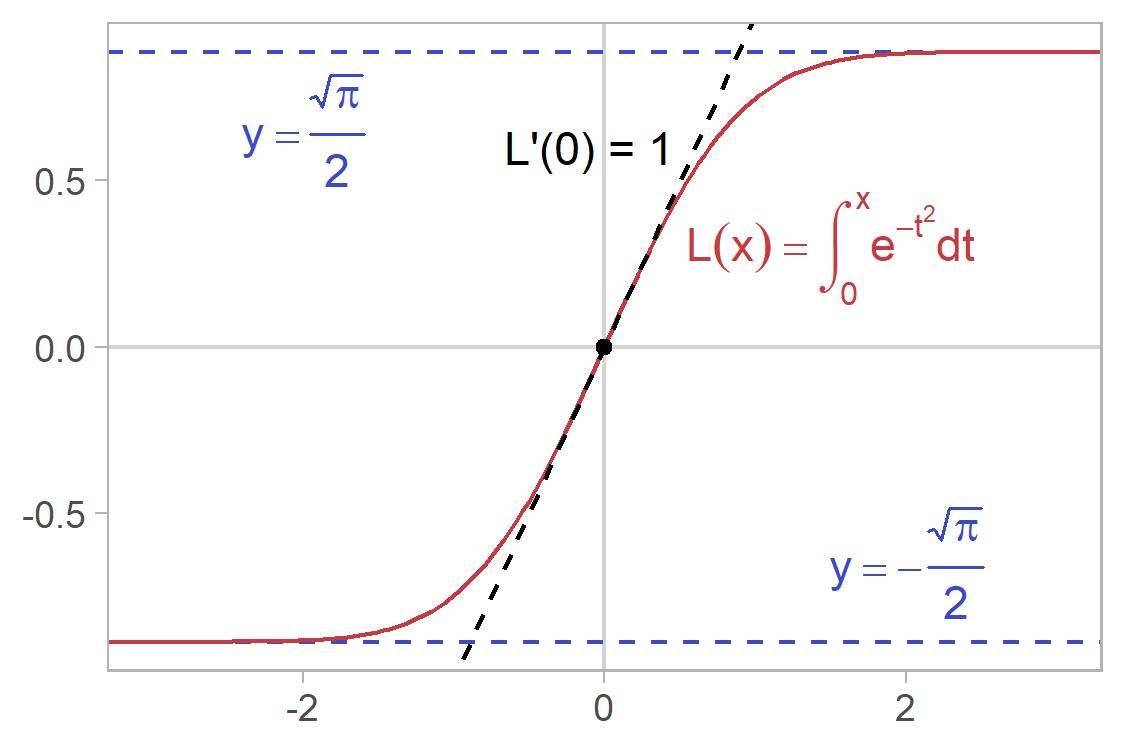
\includegraphics[scale=0.7]{img/pre_erf_plot.jpg}
\end{figure}

Una manera más rápida de haber conocido las propiedades de $L(x)$, es haber identificado que es una \textbf{función impar}:
\[
  L(-x) = -L(x)
\]
Esto se explica, primero, porque $L'(x)$ es una \textbf{función par}:
\[
  L'(-x) = L'(x)
\]
lo que geométricamente significa que es simétrica al eje vertical de un plano cartesiano.

Y, en segundo lugar, $L(x)$ es una función impar debido a que está establecido que la condición inicial de su ecuación $L'(x) = e^{-x^{2}}$ es el punto $(0, \ 0)$ o $L(0) = 0$. Recordemos que este tipo de funciones son simétricas en el origen del plano cartesiano.

Incluso lo podemos ver con el área bajo la curva de $L'(x)$, donde se cumple que $L(-x) = -L(x)$ debido a que esta derivada es una función par y a que dicha igualdad es equivalente a $\int_{0}^{-x} e^{-t^{2}}dt = -\int_{-x}^{0} e^{-t^{2}}dt$.

\begin{figure}[hbt!]
\centering
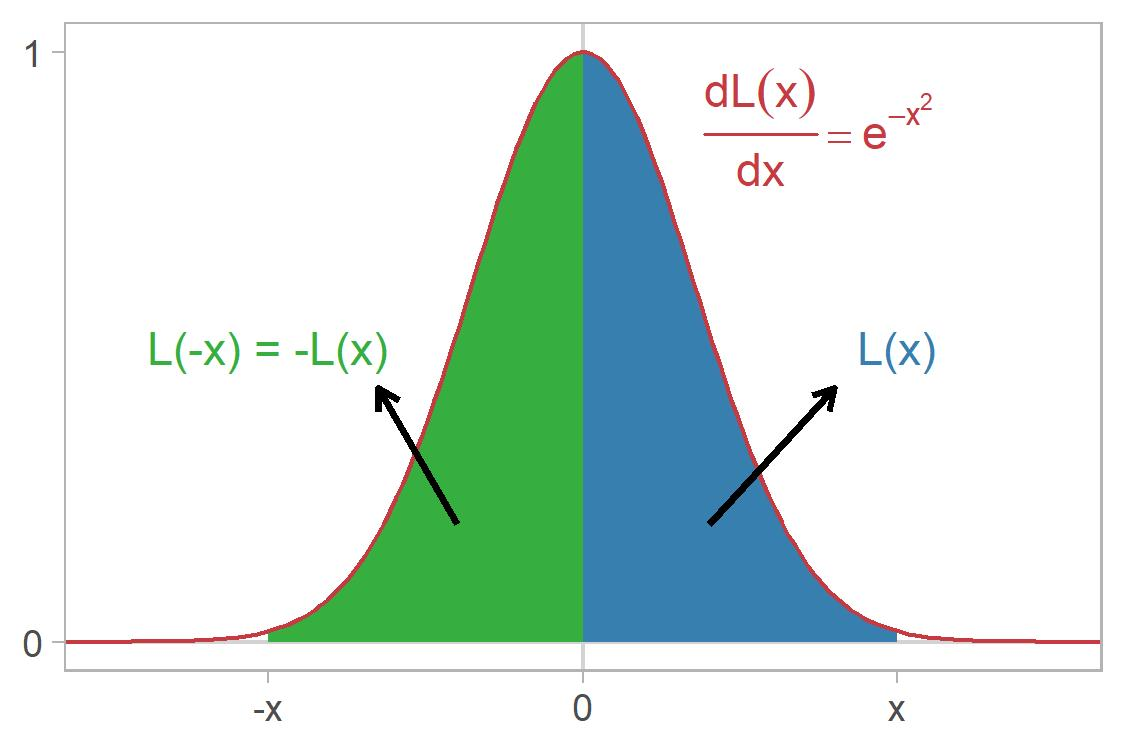
\includegraphics[scale=0.7]{img/deriv_pre_erf_plot.jpg}
\end{figure}

A partir de $L(x)$ se introdujo una nueva función, llamada \textbf{función error} y denotada como erf$(x)$, la cual es $L(x)$ siendo multiplicada por $2/\sqrt{\pi}$.
\[
  \text{erf}(x) = \frac{2}{\sqrt{\pi}} \int_{0}^{x} e^{-t^{2}}dt
\]


\section{Área entre dos curvas.}

La sección anterior aplicamos el TFC 2 para obtener funciones a partir de integrales. Ahora usaremos el TFC 1 de forma geométrica para conocer el área entre dos curvas.

Digamos que nos interesa conocer el área que se forma entre $f(x)$ y $g(x)$, las cuales son continuas para todo $x$ en $\mathbb{R}$. Existen dos métodos para lograrlo, aunque ambos se basan en la idea detrás de la suma de Riemann. Los elegimos según la estrategia que más nos convenga.

Un método es \textbf{dividir el área en rectángulos verticalmente} entre $x = a$ y $x = b$, cuyos anchos son dados por $dx$ y si $f(x) \geq g(x)$, las alturas las medimos como $f(x) - g(x)$.

\newpage

\begin{figure}[hbt!]
\centering
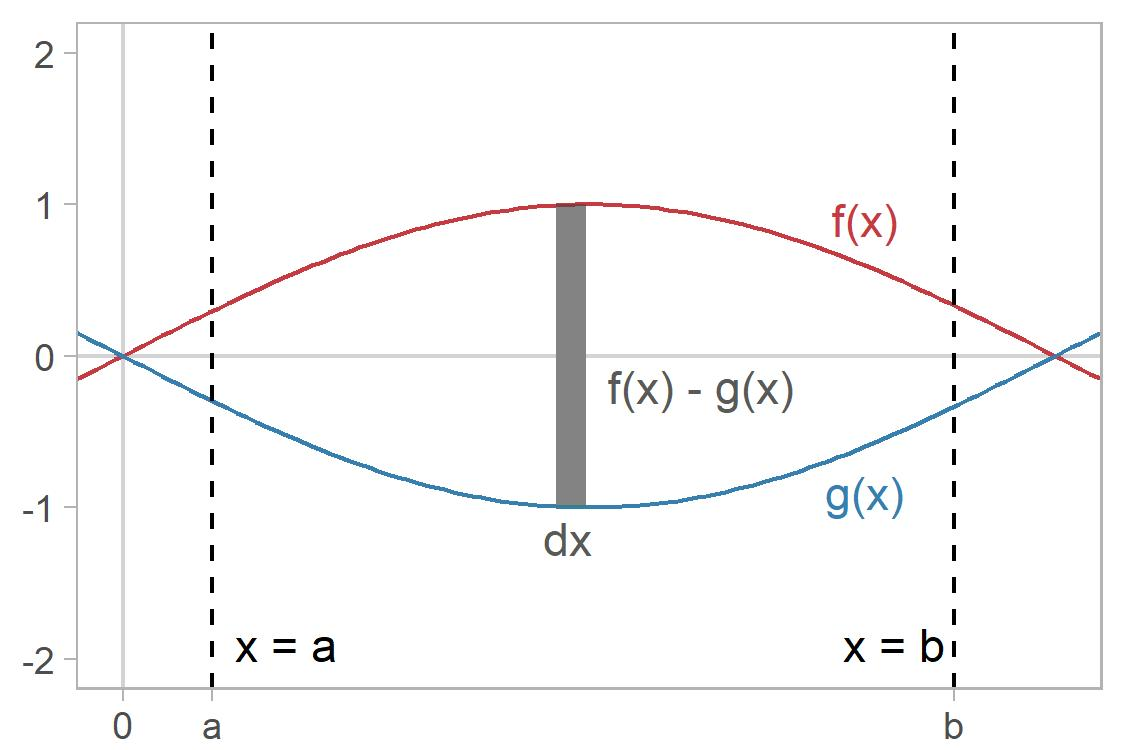
\includegraphics[scale=0.7]{img/first_method.jpg}
\end{figure}

La superficie $A$ entre las dos curvas será la \textbf{suma acumulada} del área de los rectángulos.
\[
  A = \int_{a}^{b} [f(x) - g(x)] dx
\]
En ciertas ocasiones es más conveniente calcular el área entre dos curvas usando el segundo método, que es \textbf{dividirlo horizontalmente en rectángulos} entre $y = c$ e $y = d$. Los cambios infinitesimales ahora ocurren en $y$, por lo que estará dado por $dy$ y usamos las funciones en términos de aquella variable, implicando que si $f(y) \geq g(y)$, la altura de estos cuadriláteros será $f(y) - g(y)$.

\begin{figure}[hbt!]
\centering
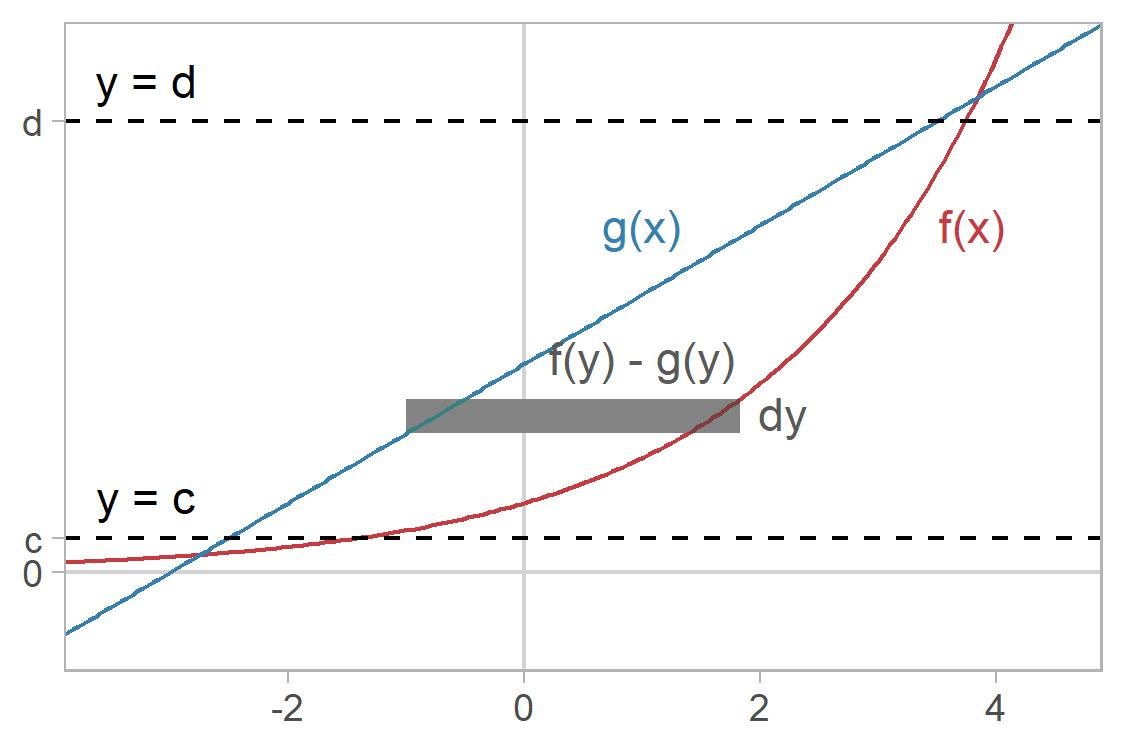
\includegraphics[scale=0.7]{img/second_method.jpg}
\end{figure}

En consecuencia, el área $A$ entre $f(x)$ y $g(x)$ se mide como la suma acumulada de las áreas de los rectángulos, pero con respecto a $y$.
\[
  A = \int_{c}^{d} [f(y) - g(y)] dy
\]
Para conocer el área entre curvas con cualquiera de los dos métodos, podemos seguir los siguientes pasos:

\begin{enumerate}
\item Dibujar las curvas.
\item Identificar el integrando y los límites de la integral ({\bf importante}).
\item Calcular la integral usando el TFC 1.
\end{enumerate}

\textbf{Ejemplo.} \quad Calcule el área que se forma entre los puntos de intersección de las funciones $x = y^{2}$ e $y = x - 2$ usando los dos métodos señalados.

\textbf{Solución.} \quad Para comenzar, veamos en qué puntos las dos funciones se intersectan o, en otras palabras, en qué valores de $y$ son iguales. Si usamos $y = x - 2$, podemos reemplazar $x$ con $x = y^{2}$, por tanto $y = y^{2} - 2$. Al igualar a cero la ecuación, entonces $0 = y^{2} - y - 2$, por lo que al factorizar el polinomio de la derecha obtenemos lo siguiente:
\[
  0 = (y - 2)(y + 1)
\]
Así, los valores de $y$ donde se intersectan ambas funciones son $y = -1$ e $y = 2$, mientras que en $x$ (usando cualquiera de las dos) son $x = 1$ y $x = 4$, respectivamente. A continuación tenemos ambas gráficas con los puntos señalados más el origen.

\begin{figure}[hbt!]
\centering
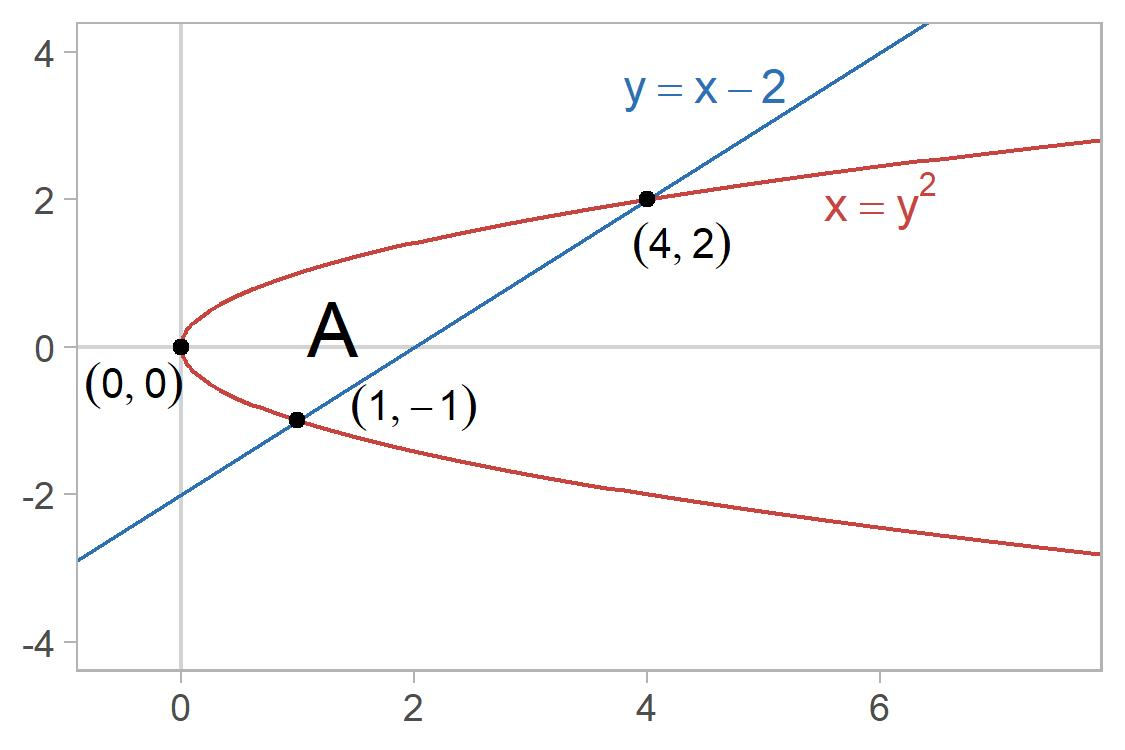
\includegraphics[scale=0.7]{img/example_init_plot.jpg}
\end{figure}

Calculemos el área $A$ comenzando con el primer método (rectángulos verticales). En este caso, las funciones deben estar en términos de $x$, por lo que en $x = y^{2}$ tendremos dos fórmulas: $y = \sqrt{x}$ e $y = -\sqrt{x}$. La dificultad es que la curva $y = -\sqrt{x}$ es tanto parte de $x = y^{2}$ como de $y = x - 2$. Por lo tanto, dividiremos $A$ en dos partes a través de $x = 1$ para evitar ese problema y después las sumaremos.

\begin{figure}[hbt!]
\centering
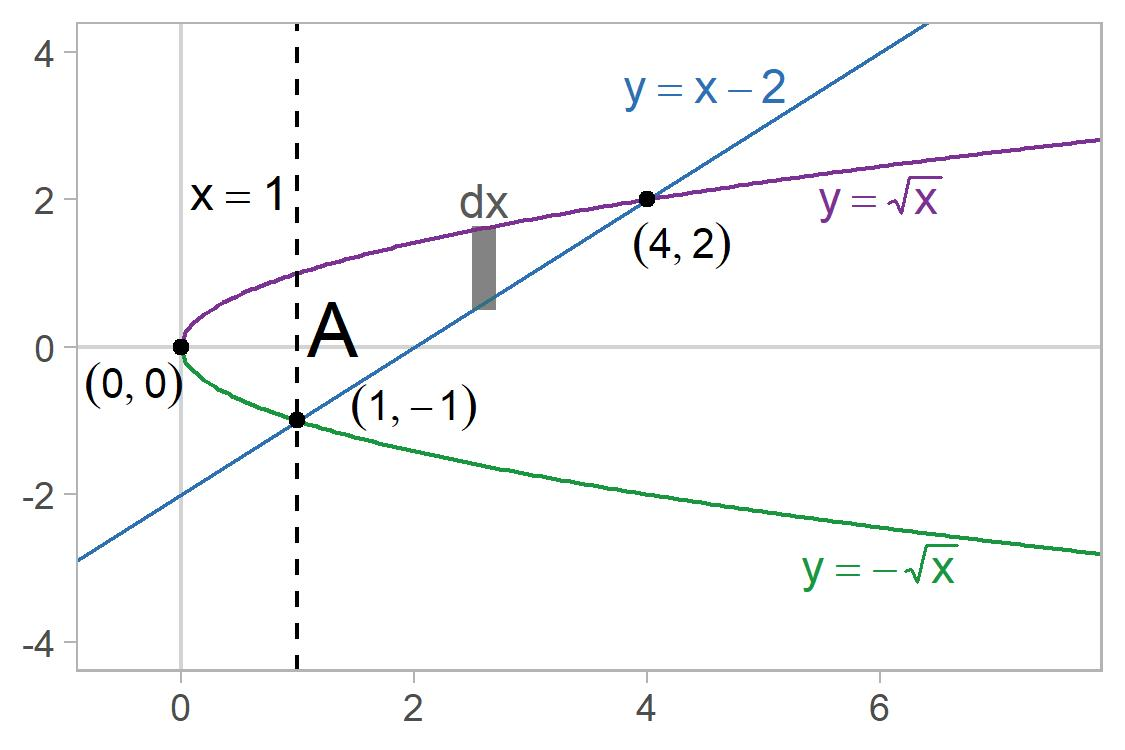
\includegraphics[scale=0.7]{img/example_method_1.jpg}
\end{figure}

Entonces, con el primer método calcularemos dos áreas: una desde $x = 0$ hasta $x = 1$ y la otra entre $x = 1$ y $x = 4$. Estos serán los límites de las dos integrales que sumaremos. Por otra parte, en la mitad izquierda las alturas de los rectángulos verticales estará dada por la diferencia entre $y = \sqrt{x}$ e $y = - \sqrt{x}$, mientras que en la derecha será entre $y = \sqrt{x}$ e $y = x - 2$. Así, el área $A$ lo calculamos como:
\[
  A = \int_{0}^{1} (\sqrt{x} - [-\sqrt{x}]) dx + \int_{1}^{4} (\sqrt{x} - [x - 2]) dx
    = 2 \cdot \left[\frac{2}{3}x^{3/2}\right]_{0}^{1} +
      \left[\frac{2}{3}x^{3/2} - \frac{x^{2}}{2} + 2x\right]_{1}^{4}
    = \frac{9}{2}
\]
Ahora usemos el \textbf{segundo método} (rectángulos horizontales). En este caso, las funciones están en términos de $y$, por lo que $y = x - 2$ la trabajamos como $x = y + 2$. Por otra parte, las alturas (anchos) de los rectángulos corresponden solo a la diferencia entre $y + 2$ e $y^{2}$ y nos movemos verticalmente entre $y = -1$ e $y = 2$, cuyos cambios (ancho vertical) están dados por $dy$.

\begin{figure}[hbt!]
\centering
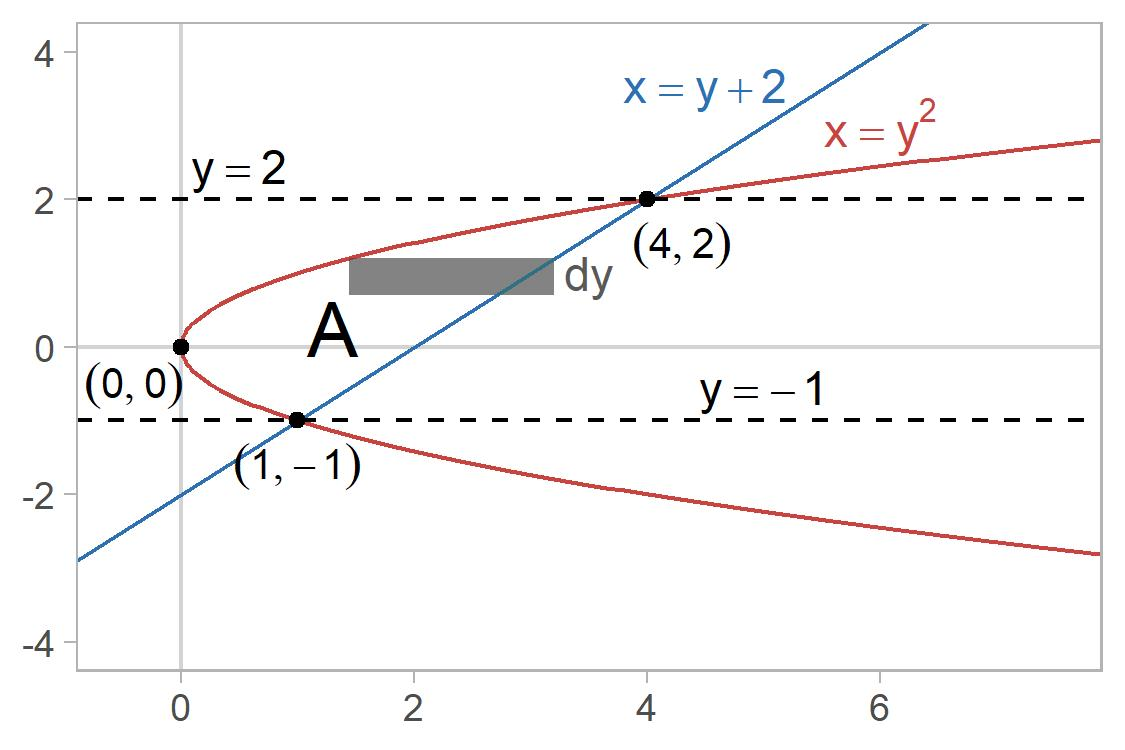
\includegraphics[scale=0.7]{img/example_method_2.jpg}
\end{figure}

Por lo tanto, el área $A$ lo calculamos como:
\[
A = \int_{-1}^{2}(y + 2 - y^{2})dy
  = \left[\frac{y^{2}}{2} + 2y - \frac{y^{3}}{3}\right]_{-1}^{2}
  = \frac{9}{2}
\]
En este ejemplo usamos ambos métodos, pero no siempre es necesario aquello. Podemos usar uno u otro, según lo que más nos convenga en el momento.

\end{document}
